%!TEX root = ../DissertationDefensePresentation.tex

%%--------------------------------------------------------------------------------------------

\subsection*{From MC Corrections}

%%--------------------------------------------------------------------------------------------

\begin{frame}
	\frametitle{Systematic Uncertainties}
	\framesubtitle{}
	\vspace*{-0.54cm}
	\begin{block}{Pileup Weights}
		\begin{itemize}
			\footnotesize
			\item Uncertainty on the weights applied to correct the pileup profile
			\item Calculated by assuming a $\pm7\%$ shift in the $\sigma_{\text{minimum bias}}$ of $69.3\unit{mb}$
			\item Shape changes are negligible for our input variables
			\item $\nu_{\text{orbit}}=$11246\unit{Hz} is the LHC orbital frequency
		\end{itemize}
		\begin{equation}
			N_{i} = \frac{\mathcal{L}\cdot\sigma_{\text{minimum bias}}}{\nu_{\text{orbit}}}
		\end{equation}
	\end{block}
	\begin{block}{Jet Energy Scale}
		\begin{columns}[T]
			\begin{column}{0.48\textwidth}
				\begin{itemize}
					\footnotesize
					\item Jets are calibrated on CMS
					\begin{itemize}
						\footnotesize
						\item The uncertainty on the calibration results in a systematic error
						\item This affects both the rate and shape of the final distributions
					\end{itemize}
					\item Each MC sample was scaled up and down by $1\sigma$ as officially prescribed
				\end{itemize}
			\end{column}
			\begin{column}{0.48\textwidth}
				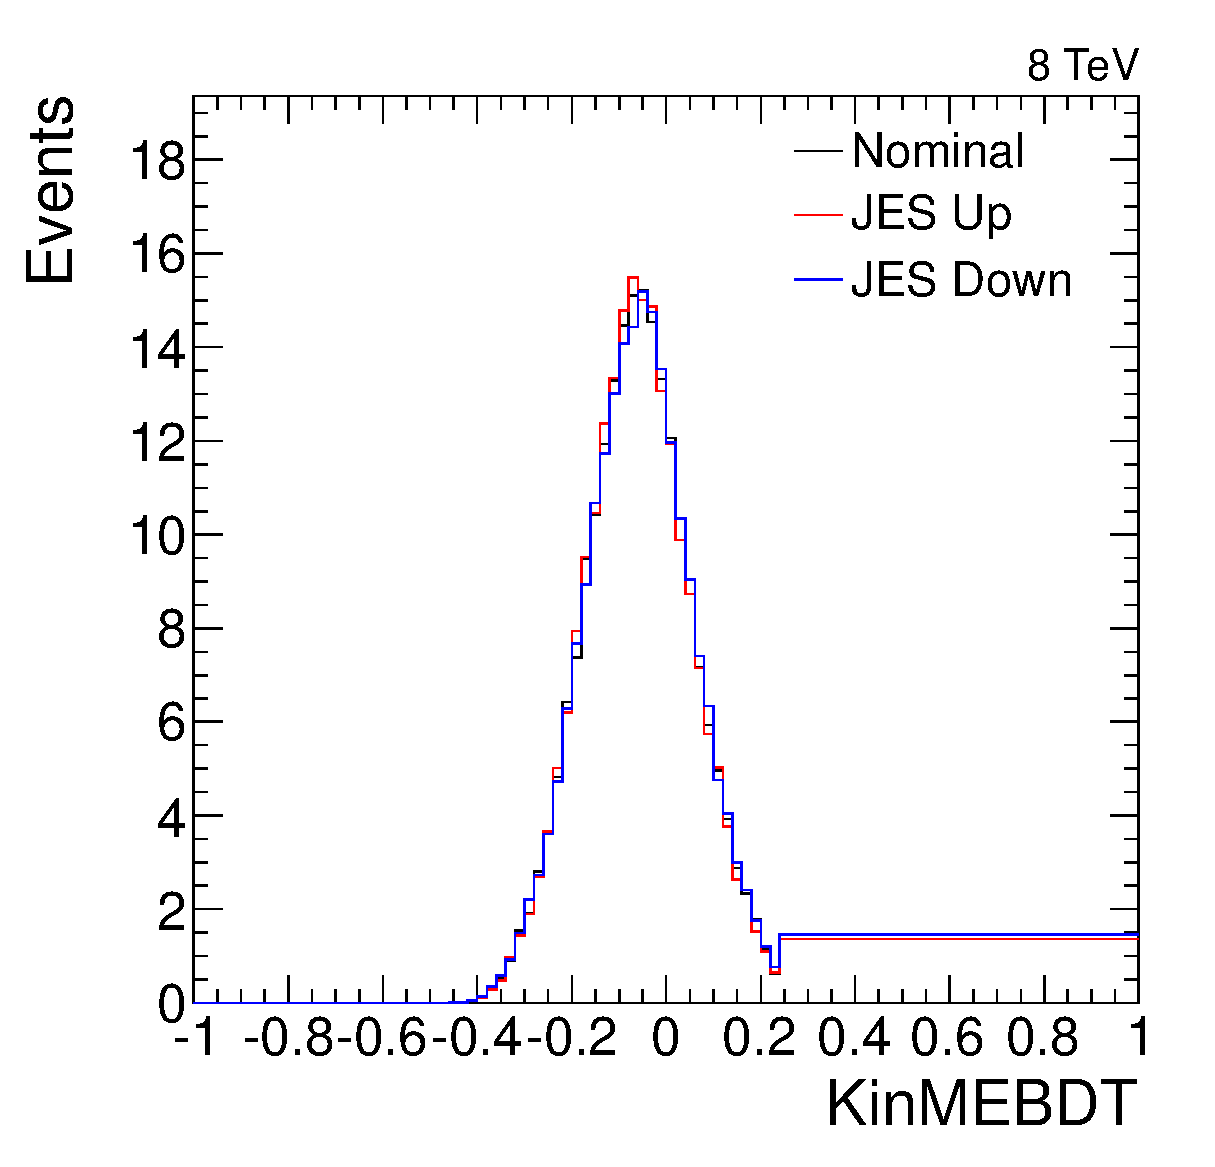
\includegraphics[width=0.49\textwidth]{\figpath/JESShift_KinMEBDT_ggH125_noCMS.eps}
				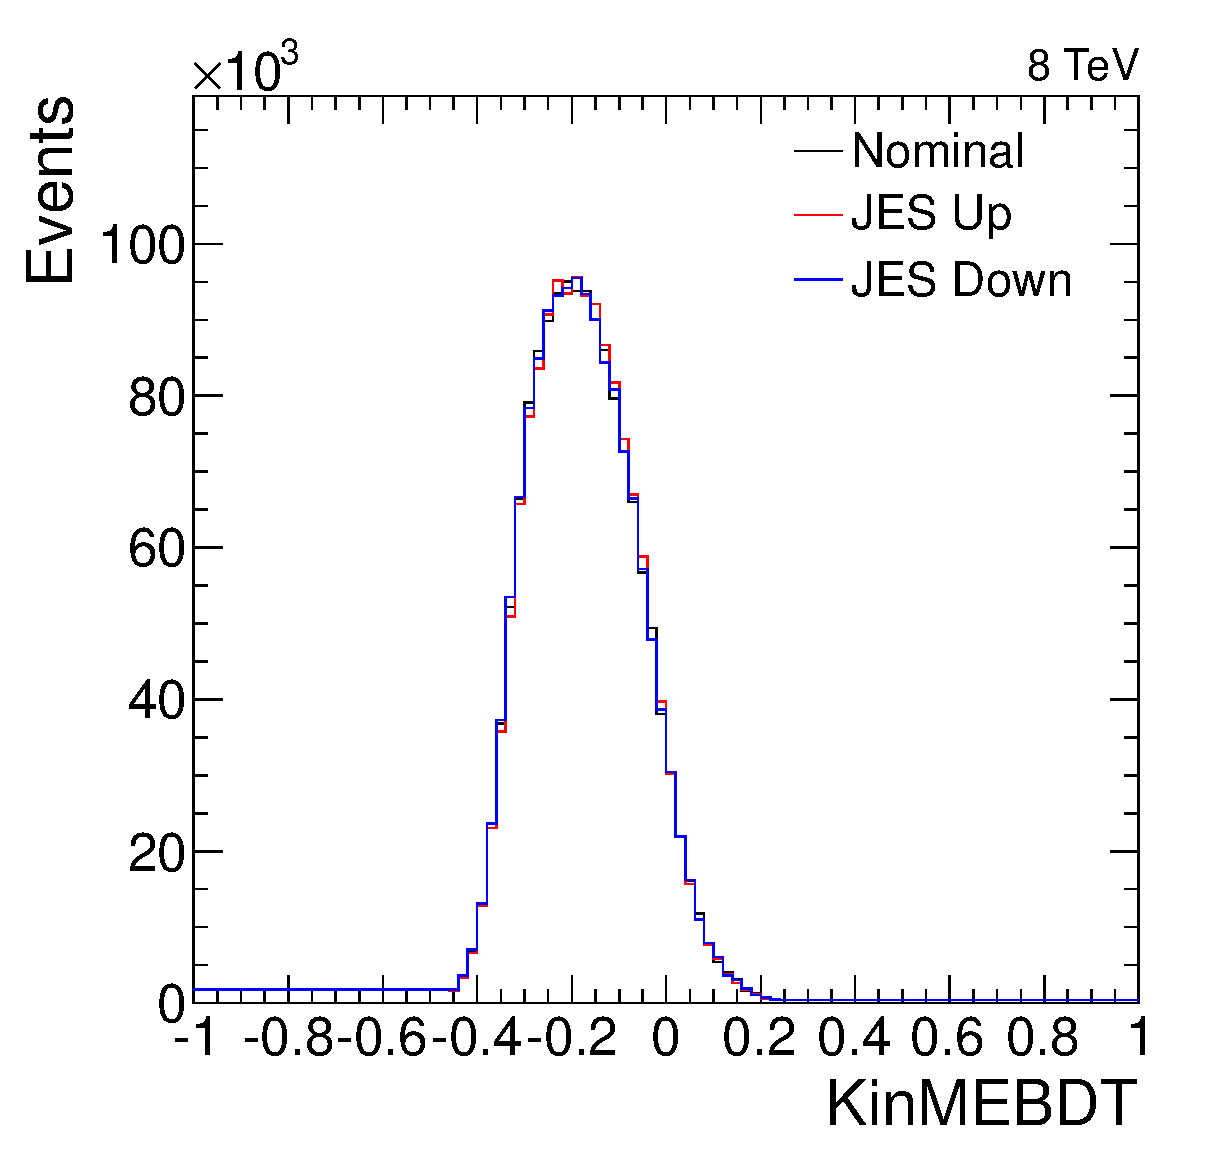
\includegraphics[width=0.49\textwidth]{\figpath/JESShift_KinMEBDT_WJets_noCMS.eps}
			\end{column}
		\end{columns}
	\end{block}
\end{frame}

%%--------------------------------------------------------------------------------------------

\subsection*{From QCD Model}

%%--------------------------------------------------------------------------------------------

\begin{frame}
	\frametitle{Systematic Uncertainties}
	\vspace*{-0.24cm}
	\begin{block}{QCD $\eta$ Weight Uncertainties}
		\begin{itemize}
			\footnotesize
			\item Generated by varying the election criteria for our data-driven QCD sample
			\item We relaxed one side of the PF isolation window and used this new selection of events to generate new $\eta$ weights
			\item Applying these new weights leads to the shape uncertainty for the QCD sample as well as rate uncertainties for the QCD (6-30\%) and \Wjets (0.1-0.5\%) samples
		\end{itemize}
	\end{block}
	\vspace*{-0.24cm}
	\begin{block}{Other Rate Uncertainties}
		\begin{itemize}
			\footnotesize
			\item Need to account for uncertainties in the \textbf{Q\textsuperscript{2} scaling and matrix element parton matching} of the dominant background (\Wjets)
			\item Systematic uncertainties due to \textbf{trigger efficiency} are on the order of 1\%
			\item Systematic uncertainties due to \textbf{lepton selection} are on the order of 2\%
			\item Uncertainty on the weights applied to correct the \textbf{b-tag discriminator} because of the b-tag veto on the events
			\item For the \textbf{top $p_{T}$ reweighting} we followed the directions of the TOP PAG
			\begin{itemize}
				\footnotesize
				%\item We use $weight^{2}$ for $\sigma_{up}$ and no weight for $\sigma_{down}$
				\item This results in a 0.5-2.1\% uncertainty on the \ttbar MC
			\end{itemize}
			\item An uncertainty of 2.6\% on the \textbf{luminosity} is applied to all MC samples
			\item PDF and $\alpha_{s}$ uncertainties for the \textbf{cross sections}
			\item Using the result from the high mass $\ell{\nu}jj$ analysis we applied a \textbf{MET uncertainty} of 0.2\%
		\end{itemize}
	\end{block}
\end{frame}

%%--------------------------------------------------------------------------------------------

\subsection*{Summary of All}
\label{sec:systematics_summary}

%%--------------------------------------------------------------------------------------------

\begin{frame}
	\frametitle{Systematic Uncertainties}
	\vspace*{-0.24cm}

\begin{table}[htbp]
	\color{black}
	\centering
  	\tiny
    \begin{tabular}{|l|c|c|l|}
		\hline
		Source                                            & Type  & Rate Uncertainty [\%] & Notes \\
		\hline
		QCD Scale (\ggH)                                  & lnN   & 7-8         & Scale uncertainty for NLO \ggH prediction \\
		QCD Scale (\qqH)                                  & lnN   & 0.2         & Scale uncertainty for NLO \qqH prediction \\
		QCD Scale (\ZH)                                   & lnN   & 1           & Scale uncertainty for NLO \ZH prediction \\
		QCD Scale (\WH)                                   & lnN   & 3.1         & Scale uncertainty for NLO \WH prediction \\
		QCD Scale (\ttH)                                  & lnN   & 4-9         & Scale uncertainty for NLO \ttH prediction \\
		\hline
		PDF ($\cPg\cPg$)                                  & lnN   & 6-7         & PDF uncertainty for $\cPg\cPg$ initiated processes (\ggH, \ttH) \\
		PDF (\qqbar)                                      & lnN   & 2.6-2.8     & PDF uncertainty for \qqbar initiated processes (\qqH, \WH, \ZH) \\
		\hline
		QCD Scale (\ttbar)                                & lnN   & 5.7         & Scale uncertainty for NLO \ttbar prediction \\
		QCD Scale (\Zjets)                                & lnN   & 3.4         & Scale uncertainty for NLO \Zjets prediction \\
		QCD Scale (Single \cPqt)                          & lnN   & 5           & Scale uncertainty for NLO single top prediction \\
		QCD Scale (\VV)                                   & lnN   & 3           & Scale uncertainty for NLO diboson prediction \\
		\hline
		\Wjets Normalization                              & lnN   & 0.4-0.5     & Scale uncertainty for \Wjets prediction \\
		QCD                                               & lnN   & 10          & Scale uncertainty for data-driven QCD prediction \\
		\ttbar                                            & lnN   & 3           & Scale uncertainty for \ttbar prediction \\
		\hline
		Luminosity $8\unit{TeV}$                          & lnN   & 2.6         & Signal and all backgrounds \\
		Lepton Efficiency                                 & lnN   & 2           & Signal and all backgrounds \\
		\ETslash                                          & lnN   & 0.2         & Signal and all backgrounds \\
		Jet Energy Scale                                  & shape & 0-20        & Signal and all backgrounds \\
		Pileup Weight                                     & shape & 0-8         & Signal and all backgrounds \\
		CSV Weight                                        & shape & 0-17        & Signal and all backgrounds \\
		Top \pt Weight                                    & shape & 0.5-2       & \ttbar only \\
		ME Matching                                       & shape & -           & \Wjets only \\
		$\text{Q}^{2}$ Scale                              & shape & -           & \Wjets only \\
		\costhetal Weight                                 & shape & -           & \Wjets only \\
		QCD Multijet $\eta$ Weight                        & shape & 6-30, 0.5-1 & QCD and \Wjets only \\
		\hline
	\end{tabular}
    \caption{Summary of the systematic uncertainties used in this analysis.}
    \label{tab:EffectOfSys}
\end{table}
\end{frame}